% \begin{name}
% 	{GV biên soạn: Duong Xuan Loi\\ GV phản biện 1: Đình Nguyên\\ GV phản biện 2: Nguyễn Sĩ Đạt}
% 	{TOÁN 10-KNTT-CS}
% \end{name}
%----------------NỘI DUNG BIÊN SOẠN
% \setcounter{chapter}{2}
\setcounter{dang}{0}
\chap{HÀM SỐ, ĐỒ THỊ VÀ ỨNG DỤNG}
\setcounter{section}{0}
\section{Hàm số}
\subsection{KIẾN THỨC TRỌNG TÂM}
\subsubsection{Khái niệm hàm số}
\begin{boxdn}\hfill
	Nếu với mỗi giá trị của $x$ thuộc tập hợp số $\mathscr{D}$ có một và chỉ một giá trị tương ứng của $y$ thuộc tập số thực $\mathbb{R}$ thì ta có một hàm số.
	\begin{enumerate}[-]
		\item Ta gọi $x$ là \textit{\textbf{biến số}} và $y$ là \textit{\textbf{hàm số}} của $x$.
		\item Tập hợp $\mathscr{D}$ được gọi là \textit{\textbf{tập xác định}} của hàm số.
		\item Tập tất cả các giá trị $y$ nhận được, gọi là \textit{\textbf{tập giá trị}} của hàm số.
	\end{enumerate}
\end{boxdn}
\begin{note}
	\begin{itemize}
	\item Khi $y$ là hàm số của $x$, ta có thể viết $y=f(x)$, $y=g(x)$, $\ldots$
	\item Khi cho hàm số bằng công thức $y=f(x)$ mà không chỉ rõ tập xác định của nó thì ta quy ước tập xác định của hàm số là tập hợp tất cả các số thực $x$ sao cho biểu thức $f(x)$ có nghĩa.
	\item Một hàm số có thể được cho bằng bảng, bằng biểu đồ, bằng công thức hoặc bằng mô tả.
	\end{itemize}
\end{note}
\subsubsection{Đồ thị của hàm số}
\begin{boxdn}	\textit{\textbf{Đồ thị của hàm số}} $y=f(x)$ xác định trên tập $\mathscr{D}$ là tập hợp tất cả các điểm $M\left(x;f(x)\right)$ trên mặt phẳng toạ độ với mọi $x$ thuộc $\mathscr{D}$.
\end{boxdn}
\subsubsection{Sự đồng biến, nghịch biến của hàm số}
\begin{boxdn}\hfill
	\begin{itemize}
		\item Hàm số $y=f(x)$ được gọi là \textit{\textbf{đồng biến (tăng)}} trên khoảng $(a;b)$, nếu
		$$\forall x_1,x_2 \in (a;b), x_1 < x_2 \Rightarrow f\left(x_1\right) < f\left(x_2\right).$$
		\item Hàm số $y=f(x)$ được gọi là \textit{\textbf{nghịch biến (giảm)}} trên khoảng $(a;b)$, nếu
		$$\forall x_1,x_2 \in (a;b), x_1 < x_2 \Rightarrow f\left(x_1\right) > f\left(x_2\right).$$
	\end{itemize}
\end{boxdn}
\begin{note}\hfill
	\begin{itemize}
		\item Đồ thị của một hàm số đồng biến trên khoảng $(a;b)$ là đường \lq\lq đi lên\rq\rq\, từ trái sang phải.
		\item Đồ thị của một hàm số đồng biến trên khoảng $(a;b)$ là đường \lq\lq đi xuống\rq\rq\, từ trái sang phải.
	\end{itemize}
\end{note}

\subsection{PHÂN LOẠI VÀ PHƯƠNG PHÁP GIẢI TOÁN}
\begin{dang}{Tìm tập xác định của hàm số}
	Để tìm tập xác định của hàm số $y=f(x)$, ta làm như sau
	\begin{itemize}
		\item Tìm điều kiện để $f(x)$ xác định.
		\item  Tập hợp các giá trị $x$ để $f(x)$ xác định là tập xác định của hàm số.
	\end{itemize}
	Một số trường hợp thường gặp
	\begin{multicols}{2}
		\begin{itemize}
			\item 	$\sqrt{f(x)}$ xác định $\Leftrightarrow f(x)\geq 0$.
			\item 	$\dfrac{1}{f(x)}$ xác định $\Leftrightarrow f(x)\neq 0$.
			\item 	$\dfrac{1}{\sqrt{f(x)}}$ xác định $\Leftrightarrow f(x)> 0$.
		\end{itemize}
	\end{multicols}
\end{dang}
\begin{vd}%[0D3N1-1]%[Biên soạn tài liệu dạy học bộ KNTT-CS]%[Duong Xuan Loi]
	Bảng sau cho biết điểm trung bình môn Toán kỳ thi tuyển sinh 10 của trường THPT A trên địa bàn TP. Hồ Chí Minh.
	\begin{center}
		\begin{tabular}[t]{|c|c|c|c|c|c|}\hline
			Thời điểm (năm)&2018&2019&2020&2021&2022\\ \hline
			Điểm trung bình môn Toán&7,24&8,02&7,65&8,14&8,34\\ \hline
		\end{tabular}
	\end{center}
	Trong bảng trên, nếu gọi $x$ là năm tuyển sinh, $y$ là điểm trung bình môn Toán của các năm thì $x$ là biến số và $y$ là hàm số của $x$. Đây là một hàm số được cho bằng bảng. Dựa vào bảng trên hãy xác định tập xác định và tập giá trị của hàm số?
	\loigiai{
		Tập xác định của hàm số là $\mathscr{D}=\{2018;2019;2020;2021;2022\}$.\\
		Tập giá trị của hàm số là $\{7,24;8,02;7,65;8,14;8,34\}$.}
\end{vd}
\begin{vd}%[0D3N1-1]%[Biên soạn tài liệu dạy học bộ KNTT-CS]%[Duong Xuan Loi]
	Viết hàm số mô tả sự phụ thuộc của quãng đường đi được vào thời gian của một vật chuyển động thẳng đều với vận tốc $3$ m/s. Tìm tập xác định của hàm số đó. Tính quãng đường vật đi được sau $10$ s, $20$ s.
	\loigiai{
		Một vật chuyển động thẳng đều với vận tốc $3$ m/s thì quãng đường đi được $S$ (mét) phụ thuộc vào thời gian $t$ (giây) theo công thức $S=3t$, trong đó $t$ là biến số, $S=S(t)$ là hàm số của $t$.\\
		Tập xác định của hàm số là $\mathscr{D}=\left[0;+\infty\right)$.\\
		Quãng đường vật đi được sau $10$ s là $S_1=S(10)=3 \cdot 10 =30$ (m).\\
		Quãng đường vật đi được sau $20$ s là $S_2=S(20)=3 \cdot 20 =60$ (m).}
\end{vd}
\begin{vd}%[0D3N1-2]%[Biên soạn tài liệu dạy học bộ KNTT-CS]%[Duong Xuan Loi]
	Tìm tập xác định của các hàm số sau
	\begin{listEX}[2]
		\item $f(x)=\sqrt{2x+7}$.
		\item $f(x)=\dfrac{x+4}{x^2-3x+2}$.
	\end{listEX}
	\loigiai{
		\begin{enumerate}
			\item Biểu thức $\sqrt{2x+7}$ có nghĩa khi $2x+7 \geq 0$, tức là $x \geq -\dfrac{7}{2}$.\\
			Vậy tập xác định của hàm số đã cho là $\mathscr{D}=\left[-\dfrac{7}{2};+\infty\right)$.
			\item Biểu thức $\dfrac{x+4}{x^2-3x+2}$ có nghĩa khi $x^2-3x+2 \ne 0$, tức là $\heva{&x \ne 1\\&x \ne 2.}$\\
			Vậy tập xác định của hàm số đã cho là $\mathscr{D}=\mathbb{R}\setminus \left\{ 1;2 \right\}$.
		\end{enumerate}
	}
\end{vd}
\begin{vd}%[0D3N1-2]%[Biên soạn tài liệu dạy học bộ KNTT-CS]%[Duong Xuan Loi]
	Tìm tập xác định và tập giá trị của mỗi hàm số sau
	\begin{listEX}[2]
		\item $ y=2x+3 $.
		\item $ y=2x^2 $.
	\end{listEX}
	\loigiai{
		\begin{enumerate}
			\item Biểu thức $ 2x+3 $ có nghĩa với mọi $ x\in \mathbb{R} $.\\
			Vậy tập xác định của hàm số đã cho là $ \mathscr{D}=\mathbb{R} $.\\
			Tập giá trị của hàm số đã cho là $ \mathbb{R} $.
			\item Biểu thức $ 2x^2 $ có nghĩa với mọi $ x\in \mathbb{R} $.\\
			Vậy tập xác định của hàm số đã cho là $ \mathscr{D}=\mathbb{R} $.\\
			Vì $ 2x^2\geq 0 $, $ \forall x\in \mathbb{R} $ nên tập giá trị của hàm số đã cho là $ [0;+\infty) $.
		\end{enumerate}
	}
\end{vd}
\begin{vd}%[0D3H1-4]%[Biên soạn tài liệu dạy học bộ KNTT-CS]%[Duong Xuan Loi]
	Tìm tập xác định của các hàm số 
	\begin{listEX}[3]
		\item $y=x^3-\dfrac{2x+1}{\sqrt{x-1}}$.
		\item $y=\sqrt[3]{2x-10}+\sqrt{9-x^2}$.
		\item $y=\dfrac{\sqrt{x+2}}{x^2+5x-6}$.
	\end{listEX}	
	\loigiai{
		\begin{enumerate}
			\item Hàm số xác định $\Leftrightarrow x-1 >0 \Leftrightarrow x>1$.\\
			Vậy tập xác định của hàm số là $\mathscr{D}=(1;+\infty)$.
			\item Hàm số xác định $\Leftrightarrow 9-x^2 \ne0 \Leftrightarrow -3\le x \le 3$.\\
			Vậy tập xác định của hàm số là $\mathscr{D}=[-3;3]$.
			\item Hàm số xác định $\Leftrightarrow \heva{&x+2 \ge 0 \\&x^2+5x-6 \ne 0} \heva{&x\ge -2\\& x \ne 1 \\&x\ne -6} \Leftrightarrow -2\le x \ne 1$.\\
			Vậy tập xác định của hàm số là $\mathscr{D}=[-2;+\infty) \setminus \{1\}$.
		\end{enumerate}		
	}
\end{vd}

\begin{dang}{Tính giá trị của hàm số tại một điểm}
	\begin{itemize}
		\item  Để tính giá trị của hàm số $f(x)$ tại $x=x_0$ ta thay thế $x$ bởi $x_0$ vào công thức $f(x)$ để tính $f(x_0)$.
		\item  Đối với các hàm số được cho bởi hai hay nhiều công thức với các miền xác định đã cho, chẳng hạn:
		$$y=f(x)=\heva{f_1(x) \text{ với } x\in \mathscr D_1 \\ f_2(x) \text{ với } x\in \mathscr  D_2}$$
		Khi tính giá trị hàm số $f(x)$ tại $x=x_0$, tùy theo $x_0$ thuộc $\mathscr D_1$ hay $\mathscr D_2$ mà ta sử dụng công thức $f(x)=f_1(x)$ hay $f(x)=f_2(x)$ để tính $f(x_0)$.
	\end{itemize}
\end{dang}
\begin{vd}%[0D3N1-4]%[Biên soạn tài liệu dạy học bộ KNTT-CS]%[Duong Xuan Loi]
	\quad
	\begin{enumerate}
		\item \immini{Cho đồ thị của hàm số $y=2x^2$ như sau, dựa vào đồ thị hàm số, hãy tìm $x$ khi $y=8$?}
		{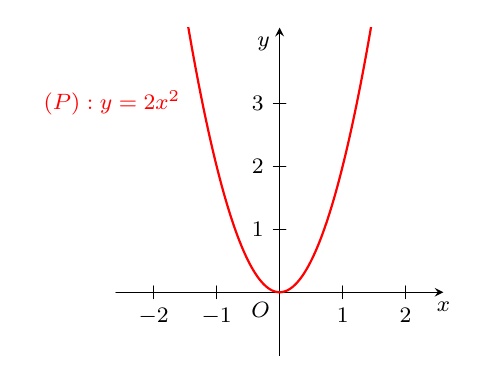
\begin{tikzpicture}[scale=0.8, font=\footnotesize, line join=round, line cap=round, >=stealth]
				\def\a{2}
				\def\b{0}
				\def\c{0}
				\def\f(#1){\a*((#1)^2)+\b*(#1)+\c}
				\def\xmin{-2.5}
				\def\xmax{2.5}
				\def\ymin{-1}
				\def\ymax{4.2}
				\clip (-4,4.2) rectangle (3,-1);
				\draw[->] (\xmin-0.1,0)--(\xmax+0.1,0) node[below] { $x$};
				\draw[->] (0,\ymin-0.1)--(0,\ymax) node[below left] { $y$};
				\draw (0,0) node [below left] { $O$};
				\foreach \x in {-2,-1,1,2}
				\draw (\x,0.1)--(\x,-0.1) node [below] { $\x$};
				\foreach \y in {1,2,3}
				\draw (0.1,\y)--(-0.1,\y) node [left] { $\y$};
				\draw[red,thick,smooth,samples=200] plot[domain=\xmin:\xmax] (\x,{\f(\x)});
				\draw (-3.9,3) node [red,right, sloped] {$(P):y=2x^2$};
		\end{tikzpicture}}
		\item Hãy vẽ đồ thị hàm số $y=2x+1$ và $y=2x^2$ trên cùng một mặt phẳng toạ độ.
	\end{enumerate}
	\loigiai{
		\begin{enumerate}
			\item Khi $y=8$ ta có $2x^2=8$, tức là $x=\pm 2$.\\
			Vậy với $x=\pm 2$ thì $y=8$.
			\item Đồ thị hàm số $y=2x+1$ và $y=2x^2$.
			\begin{center}
				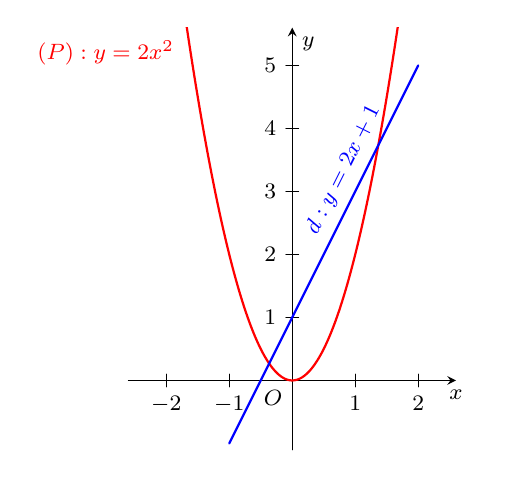
\begin{tikzpicture}[scale=0.8, font=\footnotesize, line join=round, line cap=round, >=stealth]
					\def\a{2}
					\def\b{0}
					\def\c{0}
					\def\f(#1){\a*((#1)^2)+\b*(#1)+\c}
					\def\xmin{-2.5}
					\def\xmax{2.5}
					\def\ymin{-1}
					\def\ymax{4.5}
					\clip (-4.2,5.6) rectangle (3,-1.2);
					\draw[->] (\xmin-0.1,0)--(\xmax+0.1,0) node[below] { $x$};
					\draw[->] (0,\ymin-0.1)--(0,\ymax+1.1) node[below right] { $y$};
					\draw (0,0) node [below left] { $O$};
					\foreach \x in {-2,-1,1,2}
					\draw (\x,0.1)--(\x,-0.1) node [below] { $\x$};
					\foreach \y in {1,2,3,4,5}
					\draw (0.1,\y)--(-0.1,\y) node [left] { $\y$};
					\draw[red,thick,smooth,samples=200] plot[domain=\xmin:\xmax] (\x,{\f(\x)});
					\draw [blue,thick](-1,-1)--(2,5) node [pos=0.7, above, sloped] {$d:y=2x+1$};
					\draw (-4.2,5.2) node [red,right, sloped] {$(P):y=2x^2$};
				\end{tikzpicture}
			\end{center}
		\end{enumerate}
	}
\end{vd}
\begin{vd}%[0D3N1-3]%[Biên soạn tài liệu dạy học bộ KNTT-CS]%[Duong Xuan Loi]
	Cho hàm số $f(x)=\heva{&3x-2 &\text{với } &x\ge 1 \\&1-2x^2 &\text{với } &x<1}$. Tính $f(1)$, $f(2)$, $f(0)$, $f(-3)$.
	\loigiai{
		Ta có $f(1)=1$, $f(2)=4$, $f(0)=1$, $f(-3)=-17$.
	}
\end{vd}
\begin{vd}%[0D3N1-3]%[Biên soạn tài liệu dạy học bộ KNTT-CS]%[Duong Xuan Loi]
	Cho hàm số $f(x)=\heva{&\sqrt{5-x} &\text{với } x<3 \\&\sqrt{x+5} &\text{với } x \ge 3}$. Tính $f(-4)$, $f(1)$, $f(4)$.
	\loigiai{
		Ta có  $f(-4)=3$, $f(1)=2$, $f(4)=3$.
	}
\end{vd}
\begin{vd}%[0D3N1-3]%[Biên soạn tài liệu dạy học bộ KNTT-CS]%[Duong Xuan Loi]
	Cho hàm số $f(x)=\heva{&-2x+3 &\text{với } &x<-1 \\&\, \, 3 &\text{với } &-1 \le x< 1 \\ &\sqrt{x^2-1} &\text{với } &x \ge 1}$.	Tính $f(-2)$, $f(-1)$, $f(0)$, $f(1)$, $f(2)$.
	\loigiai{
		Ta có  $f(-2)=7$, $f(-1)=3$, $f(0)=3$, $f(1)=0$, $f(2)=\sqrt{3}$.
	}
\end{vd}
\begin{vd}%[0D3N1-3]%[Biên soạn tài liệu dạy học bộ KNTT-CS]%[Duong Xuan Loi]
	Cho hàm số $f(x)=x^2-2$. Tìm giá trị của số thực $a$ sao cho $f(a-1)=2$.
	\loigiai{
		Ta có $$f(a-1)=2 \Leftrightarrow a^2-2a-1 = 2\Leftrightarrow \hoac{& a=-1\\& a=3.}$$
	}
\end{vd}
% \begin{dang}[Dùng định nghĩa xét tính đơn điệu của hàm số]
% 	Cho hàm số $y=f(x)$ xác định trên $K$ ($K$ là một khoảng hoặc một đoạn hoặc một nửa khoảng).
% 	\begin{itemize}
% 		\item[•] Hàm số $y=f(x)$ đồng biến trên $K$ khi và chỉ khi
% 		\begin{align*}
% 			&\forall x_1,x_2\in K: x_1<x_2\Rightarrow f(x_1)<f(x_2)\\
% 			\Leftrightarrow\, &\forall x_1,x_2\in K: x_1\ne x_2\Rightarrow \dfrac{f(x_1)-f(x_2)}{x_1-x_2}>0.
% 		\end{align*}
% 		\item[•] Hàm số $y=f(x)$ nghịch biến trên $K$ khi và chỉ khi
% 		\begin{align*}
% 			&\forall x_1,x_2\in K: x_1<x_2\Rightarrow f(x_1)>f(x_2)\\
% 			\Leftrightarrow\, &\forall x_1,x_2\in K: x_1\ne x_2\Rightarrow \dfrac{f(x_1)-f(x_2)}{x_1-x_2}<0.
% 		\end{align*}
% 	\end{itemize}
% \end{dang}
% \begin{vd}%[0D3N1-5]%[Biên soạn tài liệu dạy học bộ KNTT-CS]%[Duong Xuan Loi]
% 	Hãy cho biết hàm số $y=2x^2$ đồng biến hay nghịch biến trên mỗi khoảng $\left(-\infty;0 \right)$ và $\left(0;+\infty \right)$?
% 	\loigiai{
% 		\immini{Dựa vào đồ thị hàm số $y=f(x)=2x^2$
% 			\begin{itemize}
% 				\item Trên khoảng $(-\infty;0)$, đồ thị \lq\lq đi xuống\rq\rq\, từ trái sang phải và với $x_1, x_2 \in (-\infty;0), x_1 < x_2$ thì $f\left(x_1\right) > f\left(x_2\right)$. Như vậy, hàm số $y=2x^2$ nghịch biến trên khoảng $\left(-\infty;0 \right)$.
% 				\item Trên khoảng $(0;+\infty)$, đồ thị \lq\lq đi lên\rq\rq\, từ trái sang phải và với $x_3, x_3 \in (0;+\infty), x_3 < x_4$ thì $f\left(x_3\right) < f\left(x_4\right)$. Như vậy, hàm số $y=2x^2$ đồng biến trên khoảng $\left(0;\infty \right)$.
% 			\end{itemize}
% 		}{\begin{tikzpicture}[scale=0.8, font=\footnotesize, line join=round, line cap=round, >=stealth]
% 				\def\a{2}
% 				\def\b{0}
% 				\def\c{0}
% 				\def\f(#1){\a*((#1)^2)+\b*(#1)+\c}
% 				\def\xmin{-2.5}
% 				\def\xmax{2.5}
% 				\def\ymin{-1}
% 				\def\ymax{4.5}
% 				\clip (-2.5,5.6) rectangle (3,-1);
% 				\draw[->] (\xmin-0.1,0)--(\xmax+0.1,0) node[below] { $x$};
% 				\draw[->] (0,\ymin-0.1)--(0,\ymax+1.1) node[below right] { $y$};
% 				\draw (0,0) node [below left] { $O$};
% 				\draw[dashed] (-1.4,0) node[below]{$x_1$}--(-1.4,3.92)--(0,3.92) node[right]{$f\left(x_1\right)$}
% 				(-0.75,0)node[below]{$x_2$}--(-0.75,1.125)--(0,1.125) node[right]{$f\left(x_2\right)$}
% 				(1,0)node[below left]{$x_3$}--(1,2)--(0,2) node[left]{$f\left(x_3\right)$}
% 				(1.2,0)node[below right]{$x_4$}--(1.2,2.88)--(0,2.88) node[left]{$f\left(x_4\right)$};
% 				\draw[thick,->] (-1.8,5)--(-1.6,3.92);
% 				\draw[thick,->] (1.6,3.92)--(1.8,5);
% 				\draw[blue,thick,smooth,samples=200] plot[domain=\xmin:0] (\x,{\f(\x)});
% 				\draw[red,thick,smooth,samples=200] plot[domain=0:\xmax] (\x,{\f(\x)});
% 				\draw (-1.6,5.2) node [red,right, sloped] {$y=2x^2$};
% 		\end{tikzpicture}}
% 	}
% \end{vd}
% \begin{vd}%[0D3H1-5]%[Biên soạn tài liệu dạy học bộ KNTT-CS]%[Duong Xuan Loi]
% 	Dùng định nghĩa xét tính đồng biến và nghịch biến của hàm số $y=x^2+10x+9$ trên $(-5;+\infty)$.
% 	\loigiai{
% 		Gọi $x_1$, $x_2$ là hai giá trị phân biệt tùy ý thuộc $(-5;+\infty)$, ta có
% 		$$\dfrac{f(x_1)-f(x_2)}{x_1-x_2}=\dfrac{(x_1^2+10x_1+9)-(x_2^2+10x_2+9)}{x_1-x_2}=\dfrac{(x_1-x_2)(x_1+x_2+10)}{x_1-x_2}=x_1+x_2+10.$$
% 		Do $x_1>-5, x_2>-5$ nên $x_1+x_2>-10\Leftrightarrow x_1+x_2+10>0$. Suy ra $\dfrac{f(x_1)-f(x_2)}{x_1-x_2}>0$.\\
% 		Vậy hàm số đồng biến trên khoảng $(-5;+\infty)$.
% 	}
% \end{vd}
% \begin{vd}%[0D3H1-5]%[Biên soạn tài liệu dạy học bộ KNTT-CS]%[Duong Xuan Loi]
% 	Dùng định nghĩa xét tính đơn điệu của hàm số $y=\dfrac{1+x}{1-x}$ trên $(-\infty;1)$.
% 	\loigiai{
% 		Gọi $x_1, x_2$ là hai giá trị phân biệt tùy ý thuộc $(-\infty;1)$, ta có
% 		$$\dfrac{f(x_1)-f(x_2)}{x_1-x_2}=\dfrac{\dfrac{1+x_1}{1-x_1}-\dfrac{1+x_2}{1-x_2}}{x_1-x_2}=\dfrac{2}{(1-x_1)(1-x_2)}.$$
% 		Do $x_1<1, x_2<1$ nên $(1-x_1)(1-x_2)>0$, từ đó suy ra $\dfrac{f(x_1)-f(x_2)}{x_1-x_2}>0$.\\
% 		Vậy hàm số đã cho đồng biến trên $(-\infty;1)$.
% 	}
% \end{vd}
% \begin{vd}%[0D3H1-5]%[Biên soạn tài liệu dạy học bộ KNTT-CS]%[Duong Xuan Loi]
% 	Dùng định nghĩa xét sự biến thiên của hàm số $y=\sqrt{x-1}$ trên tập xác định.
% 	\loigiai{
% 		Tập xác định $\mathscr{D}=[1;+\infty)$.\\
% 		Gọi $x_1$, $x_2$ là hai giá trị phân biệt tùy ý thuộc $[1;+\infty)$, ta có
% 		$$\dfrac{f(x_1)-f(x_2)}{x_1-x_2}=\dfrac{\sqrt{x_1-1}-\sqrt{x_2-1}}{x_1-x_2}=\dfrac{1}{\sqrt{x_1-1}+\sqrt{x_2-1}}>0.$$
% 		Vậy hàm số đã cho luôn đồng biến trên tập xác định.
% 	}
% \end{vd}
% \begin{vd}%[0D3H1-5]%[Biên soạn tài liệu dạy học bộ KNTT-CS]%[Duong Xuan Loi]
% 	Dùng định nghĩa xét sự biến thiên của hàm số $y=|x-3|$ trên tập xác định.
% 	\loigiai{
% 		Tập xác định $\mathscr{D}=\mathbb{R}$.\\
% 		Với mọi  $x_1$, $x_2\in \mathbb{R}$, $x_1\ne x_2$, ta có  $$\dfrac{f(x_1)-f(x_2)}{x_1-x_2}=\dfrac{|x_1-3|-|x_2-3|}{x_1-x_2}.$$
% 		\begin{itemize}
% 			\item Với $x_1, x_2\in (-\infty;3)$ thì $\dfrac{f(x_1)-f(x_2)}{x_1-x_2}=\dfrac{(3-x_1)-(3-x_2)}{x_1-x_2}=-1<0$.\\
% 			Từ đó suy ra hàm số nghịch biến trên $(-\infty;3)$.
% 			\item Với $x_1, x_2\in (3;+\infty)$ thì $\dfrac{f(x_1)-f(x_2)}{x_1-x_2}=\dfrac{(x_1-3)-(x_2-3)}{x_1-x_2}=1>0$.\\
% 			Từ đó suy ra hàm số đồng biến trên $(3;+\infty)$.
% 		\end{itemize}
% 		Bảng biến thiên
% 		\begin{center}
% 			\begin{tikzpicture}
% 				\tkzTabInit[nocadre=true,lgt=0.7,espcl=3.5]{$x$ /0.7,$y$ /2}
% 				{$-\infty$,3,$+\infty$}
% 				%\tkzTabLine{,-,0,+,0,-,}
% 				\tkzTabVar{+/$+\infty$/,-/$0$/,+/$+\infty$/}
% 			\end{tikzpicture}
% 		\end{center}
% 	}
% \end{vd}
\begin{dang}{Dùng đồ thị xét tính đơn điệu của hàm số}
	Cho hàm số $y=f(x)$ xác định trên $K$ ($K$ là một khoảng hoặc một đoạn hoặc một nửa khoảng).
	\begin{itemize}
		\item  Hàm số đồng biến trên $K$ khi và chỉ khi đồ thị hàm số \lq\lq đi lên\rq\rq\;trên $K$.
		\item Hàm số nghịch biến trên $K$ khi và chỉ khi đồ thị hàm số \lq\lq đi xuống\rq\rq\; trên $K$.
		\item Khi nói đồ thị \lq\lq đi lên\rq\rq\; hay \lq\lq đi xuống\rq\rq, ta luôn kể theo chiều tăng của biến số, nghĩa là kể từ trái qua phải.
	\end{itemize}
\end{dang}
\begin{vd}%[0D3N1-5]%[Biên soạn tài liệu dạy học bộ KNTT-CS]%[Duong Xuan Loi]
	\immini{Cho hàm số $y=f(x)$ có đồ thị như hình vẽ bên. Tìm các khoảng đồng biến, các khoảng nghịch biến của hàm số.}{
		\begin{tikzpicture}[>=stealth,line join=round,line cap=round,font=\footnotesize,scale=0.7]
			\def\a{1} \def\b{4} \def\c{3} % Hệ số
			\def\xt{-5} \def\xp{3} \def\yt{4} \def\yd{-2} % x_trái, x_phải, y_trên, y_dưới (giới hạn)
			\draw[->] (\xt,0)--(\xp,0) node [below]{$x$};
			\draw[->] (0,\yd)--(0,\yt) node [left]{$y$};
			\node at (0,0) [below left]{$O$};
			\draw[dashed] (-2,0)--(-2,-1)--(0,-1) node [right]{$-1$};
			\node at (-2,0) [above]{$-2$};
			\node at (0,3) [right]{$3$};
			\clip (\xt-0.1,\yd+0.1) rectangle (\xp-0.1,\yt-0.1);
			\draw[smooth,samples=300] plot(\x,{\a*(\x)^2+\b*(\x)+\c});
			\fill (0,0) circle(1pt)(-2,0) circle(1pt)(0,3) circle(1pt)(0,-1) circle(1pt)(-2,-1) circle(1pt);
	\end{tikzpicture}}
	\loigiai{
		Từ đồ thị, ta có hàm số đồng biến trên khoảng $(-2;+\infty)$ và nghịch biến trên khoảng $(-\infty;-2)$.}
\end{vd}
\begin{vd}%[0D3N1-5]%[Biên soạn tài liệu dạy học bộ KNTT-CS]%[Duong Xuan Loi]
	\immini{Cho hàm số $y=f(x)$ có đồ thị như hình vẽ bên. Tìm các khoảng đồng biến, các khoảng nghịch biến của hàm số.}{
		\begin{tikzpicture}[>=stealth,line join=round,line cap=round,font=\footnotesize,scale=1]
			\draw[->] (0,-1)--(0,1) node[left]{$1$}--(0,2)node[left]{$2$} -- (0,4.5) node[left]{$y$};
			\draw[->] (-1,0)--(0,0) node[below left]{$O$}--(1,0) node[below ]{$1$}--(2,0)node[below]{$2$}-- (3.5,0) node[below]{$x$};
			\draw[-][dashed] (0,2)--(1,2) (0,1)--(2,1)--(2,0) (1,0)--(1,2);
			\draw[-][smooth,samples=600,domain=2:3] plot(\x,{(\x)^2-2*(\x)+1});
			\draw[-][smooth,samples=600,domain=-1:0] plot(\x,{(\x)^2-2*(\x)+1});
			\draw[-][smooth,samples=100,domain=0:2] plot(\x,{-(\x)^2+2*(\x)+1});
			\fill (1,0) circle(1pt) (2,0) circle(1pt)
			(0,1) circle(1pt) (0,2) circle(1pt)
			(1,2) circle(1pt)(2,1) circle(1pt);
	\end{tikzpicture}}
	\loigiai{Từ đồ thị, ta có hàm số đồng biến trên các khoảng $(0;1)$, $(2;+\infty)$, nghịch biến trên khoảng $(-\infty;0)$, $(1;2)$.}
\end{vd}
\begin{vd}%[0D3N1-5]%[Biên soạn tài liệu dạy học bộ KNTT-CS]%[Duong Xuan Loi]
	\immini{Cho hàm số $y=f(x)$ xác định trên $(-6;+\infty)$, có đồ thị như hình vẽ bên. Tìm các khoảng đồng biến, các khoảng nghịch biến của hàm số.
	}{
		\begin{tikzpicture}[>=stealth,line join=round,line cap=round,font=\footnotesize,scale=0.6]
			\draw[-> ] (-6.5,0) -- (2,0)node[below] {$x$};
			\draw[-> ] (0,-1.0) -- (0,11)node[right] {$y$};
			\draw(0,0) node[below left=-0.05] {$O$};
			\draw[red,smooth,samples=100,domain=-3:1.12]  plot (\x,{(\x)^2+4*(\x)+5});
			\draw[red] (-6,2)--(-3,2);
			\draw[dashed] (-6,0)node[below]{$-6$}--(-6,2) (-3,0)node[below]{$-3$}--(-3,2)--(0,2)node[right]{$2$};
			\draw[dashed](-2,0)node[below]{$-2$}--(-2,1)--(0,1)node[right]{$1$};
			\draw (0,5)node[right]{$5$};
			\draw[dashed](1,0)node[below]{$1$}--(1,10)--(0,10)node[left]{$10$};
			\fill (-6,0) circle(1pt) (-3,0) circle(1pt) (-2,0) circle(1pt) (-6,2) circle(1pt)(-3,2) circle(1pt)
			(-2,1) circle(1pt)
			(1,10) circle(1pt)
			(-2,-1) circle(1pt)(0,1) circle(1pt)(0,2) circle(1pt)
			(0,5) circle(1pt);
	\end{tikzpicture}}
	\loigiai{Từ đồ thị, ta có hàm số không đổi trên $(-6;-3)$, nghịch biến trên $(-3;-2)$ và đồng biến trên $(-2;+\infty)$.}
\end{vd}
\begin{vd}%[0D3N1-5]%[Biên soạn tài liệu dạy học bộ KNTT-CS]%[Duong Xuan Loi]
	\immini{Cho hàm số $y=f(x)$ có đồ thị như hình vẽ bên.
		\begin{enumerate}
			\item Tìm các khoảng đồng biến, các khoảng nghịch biến của hàm số.
			\item Tìm giá trị lớn nhất, giá trị nhỏ nhất của hàm số trên đoạn $\left[0; 2\right]$.
	\end{enumerate}}{
		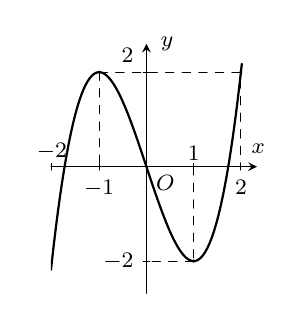
\begin{tikzpicture}[>=stealth,line join=round,line cap=round,font=\footnotesize,scale=0.6]
			\draw[->,color=black] (-2.02,0.) -- (2.34,0.);
			\foreach \x in {-1,2}
			\draw[shift={(\x,0)},color=black] (0pt,2pt) -- (0pt,-2pt) node[below] {$\x$};
			\foreach \x in {-2,1}
			\draw[shift={(\x,0)},color=black] (0pt,2pt) -- (0pt,-2pt) node[above] {$\x$};
			\draw[color=black] (2.02,0.08) node [anchor=south west] {$x$};
			\draw[->,color=black] (0.,-2.68) -- (0.,2.6);
			\foreach \y in {-2}
			\draw[shift={(0,\y)},color=black] (2pt,0pt) -- (-2pt,0pt) node[left] {$\y$};
			\foreach \y in {2}
			\draw[shift={(0,\y)},color=black] (2pt,0pt) -- (-2pt,0pt) node[above left] {$\y$};
			\draw[color=black] (0.1,2.6) node [anchor=west] { $y$};
			\draw[color=black] (0pt,-10pt) node[right] {$\tiny  {\text{O}}$};
			\clip(-2.02,-2.68) rectangle (2.34,2.66);
			\draw[smooth][line width=0.8pt,color=black,smooth,samples=100,domain=-2.02:2.02] plot(\x,{(\x^3.0-3.0*\x});
			\draw [dashed] (-1.,2.)-- (0,2)--(2,2)--(2,0);
			\draw [dashed] (-1.,2.)-- (-1.,0.);
			\draw [dashed] (1.,0.)-- (1.,-2.);
			\draw [dashed] (1.,-2.)-- (0.,-2.);
			\fill (1,-2) circle(1pt)
			(-1,2) circle(1pt)(2,2) circle(1pt);
	\end{tikzpicture}}
	\loigiai{
		\begin{enumerate}
			\item
			Từ đồ thị, ta có hàm số đồng biến trên các khoảng $(-\infty; -1)$ và $(1; +\infty)$, nghịch biến trên khoảng $(-1;1)$.
			\item Từ đồ thị ta thấy trên đoạn $[0;2]$ hàm số đã cho có giá trị nhỏ nhất bằng $-2$ và giá trị nhỏ nhất bằng $2$.
	\end{enumerate}}
\end{vd}
\begin{dang}{Bài toán thực tế}
\end{dang}
\begin{vd}%[0D3V1-7]%[Biên soạn tài liệu dạy học bộ KNTT-CS]%[Duong Xuan Loi]
	Bảng giá nước đối tượng sinh hoạt ở thành phố H năm 2021 được cho như bảng dưới đây
	\begin{center}
		\scalebox{0.85}{
			\begin{tabular}{|c|c|c|c|}
				\hline
				Mức sử dụng (m$^3$/tháng/1 người)  & Giá chưa thuế GTGT (VNĐ/ m$^3$)& Phí BVMT&Thuế GTGT\\
				\hline
				Từ $0$ đến $4$ m$^3$  & $5\,300$ &$530$&$265$\\
				\hline
				Từ trên $4$ m$^3$ đến $6$ m$^3$  & $10\,200$ &$1\,020$&$510$\\
				\hline
				Trên $6$ m$^3$  & $11\,400$& $1\,140$ &$570$\\
				\hline
			\end{tabular}
		}
	\end{center}
	Hãy tính số tiền phải trả ứng với mỗi mức sử dụng nước ở bảng dưới đây.
	\begin{center}
		\scalebox{1}{
			\begin{tabular}{|c|c|c|c|}
				\hline
				Mức sử dụng (m$^3$)  & $ 3 $& $ 5{,}5 $ & $ 7 $\\
				\hline
				Số tiền (nghìn đồng)  &  & & \\
				\hline
			\end{tabular}
		}
	\end{center}
	\loigiai{
		Tổng số tiền $ T $ phải trả là một hàm số của $ x $ m$^3 $ nước.\\
		Ta có $ T(3) =3\cdot (5\,300+530+265)= 18\,285$,\\
		$ T(5{,}5) =4\cdot (5\,300+530+265)+1{,}5\cdot (10\,200+1\,020+510)=41\,975$,\\
		$ T(7) =4\cdot (5\,300+530+265)+2\cdot (10\,200+1\,020+510)+(11\,400+1\,140+570)=60\,950$.\\
		Do đó ta được bảng dưới đây.
		\begin{center}
			\scalebox{1}{
				\begin{tabular}{|c|c|c|c|}
					\hline
					Mức sử dụng (m$^3$)  & $ 3 $& $ 5{,}5 $ & $ 7 $\\
					\hline
					Số tiền (nghìn đồng)  & $ 18\,285 $ & $ 41\,975 $ &$ 60\,950 $ \\
					\hline
				\end{tabular}
			}
		\end{center}
	}
\end{vd}
\begin{vd}%[0D3V1-7]%[Biên soạn tài liệu dạy học bộ KNTT-CS]%[Duong Xuan Loi]
	Theo quyết định số $ 2019$/QĐ-BĐVN  ngày $ 01/01/2018 $ của Tổng công ty Bưu điện Việt Nam, giá cước dịch vụ Bưu chính phổ cập đối với dịch vụ thư cơ bản và bưu thiếp trong nước có khối lượng đến $ 250 $ g như trong bảng sau
	\immini{
		\begin{enumerate}
			\item Số tiền dịch vụ thư cơ bản phải trả $ y $ (đồng) có là hàm số của khối lượng thư cơ bản $ x $ (g) hay không? Nếu đúng hãy xác định những công thức tính $ y $.
		\end{enumerate}
	}{
		\begin{tabular}[t]{|c|c|}
			\hline
			\textbf{Khối lượng đến} $ 250 $ g & \textbf{Mã cước (đồng)} \\
			\hline
			\textbf{Đến} $ 20 $ g & $4\,000$ \\
			\hline
			\textbf{Trên} $ 20 $ g \textbf{đến} $ 100 $ g & $6\,000$\\
			\hline
			\textbf{Trên} $ 100 $ g \textbf{đến} $ 250 $ g & $8\,000$\\
			\hline
		\end{tabular}
	}
	\begin{enumerate}
		\item [b)] Tính số tiền phải trả khi bạn Dương gửi thư có khối lượng $ 150 $ g, $ 200 $ g.
	\end{enumerate}
	\loigiai{
		\begin{enumerate}
			\item Ta có $ y $ là một hàm số theo $ x $.\\
			$y= \heva{&4\,000x&(x\leq 20)\\&4\,000\cdot 20+(x-20)\cdot 6\,000&(20<x\leq 100)\\&4\,000\cdot 20+6\,000\cdot 80+(x-100)\cdot 8\,000&(100<x\leq 250)} \\
			\Leftrightarrow y= \heva{&4\,000x&(x\leq 20)\\&6\,000x-40\,000&(20<x\leq 100)\\& 8\,000x-240\,000&(100<x\leq 250).} $
			\item Bạn Dương gửi thư có khối lượng
			\begin{itemize}
				\item $ 150 $ g số tiền phải trả là $ y=8\,000\cdot 150-240\,000=960\,000 $ đồng.
				\item $ 200 $ g số tiền phải trả là $ y=8\,000\cdot 200-240\,000=1\,360\,000 $ đồng.
			\end{itemize}
		\end{enumerate}
	}
\end{vd}
\begin{vd}%[0D3V1-7]%[Biên soạn tài liệu dạy học bộ KNTT-CS]%[Duong Xuan Loi]
	Một lớp học thuê một hướng dẫn viên cho chuyến tham quan, có hai công ty được liên hệ  để tham khảo giá.
	\begin{itemize}
		\item Công ty $ A $ có phí dịch vụ ban đầu là $ 400 $ nghìn đồng cộng thêm $ 3\,000 $ đồng cho mỗi ki-lô-mét hướng dẫn.
		\item Công ty $ B $ có phí dịch vụ ban đầu là $ 300 $ nghìn đồng cộng thêm $ 3 $ nghìn $ 500 $ đồng cho mỗi ki-lô-mét hướng dẫn.
	\end{itemize}
	\begin{enumerate}
		\item Lớp học nên chọn công ty nào để thuê hướng dẫn viên nếu biết rằng chuyến đi sẽ đến một địa điểm nào đó với tổng khoảng cách đi lại là $ 250 $ km.
		\item Nếu đi khoảng cách là bao nhiêu thì chọn công ty $ A $ có lợi hơn.
	\end{enumerate}
	\loigiai{
		Gọi $ x $	là số km lớp đó đi ($ x>0 $).\\
		Số tiền phải trả cho công ty $ A $ là $ 400+3x $ (nghìn đồng).\\
		Số tiền phải trả cho công ty $ B $ là $ 300+3{,}5x $ (nghìn đồng).
		\begin{enumerate}
			\item Nếu $ x=250 $ km thì  số tiền phải trả cho công ty $ A $ là $ 400+3\cdot 250=1\,150 $ (nghìn đồng), số tiền phải trả cho công ty $ B $ là $ 300+3{,}5\cdot 50=1\,175 $ (nghìn đồng).\\
			Vậy chọn công ty $ A $ có lợi  hơn.
			\item Chọn công ty $ A $ có lợi hơn tức số tiền phải trả cho công ty $ A $ ít hơn số tiền phải trả cho công ty $ B $. Ta có bất phương trình $ 400+3x<300+3{,}5x\Leftrightarrow x>200$.\\
			Vậy chọn công ty $ A $ lợi hơn nếu tổng khoảng cách đi lại lớn hơn $ 200 $ km.
		\end{enumerate}
	}
\end{vd}
%%%%%%%%%%%%%%%%%%%%%%%%%%%%%%%%%%%%%
\subsection{BÀI TẬP RÈN LUYỆN}
%-------------Trắc nghiệm nhiều lựa chọn
\ind{PHẦN I.} \inden{Câu trắc nghiệm nhiều phương án lựa chọn. Mỗi câu hỏi học sinh chỉ chọn một phương án.}
\setcounter{ex}{0}
\Opensolutionfile{ans}[ans/ans-c6b15-lc]
\begin{ex}%[0D3N1-4]%[Biên soạn tài liệu dạy học bộ KNTT-CS]%[Duong Xuan Loi]
	Cho hàm số $y = \dfrac{x + 1}{x - 1}$. Tìm tọa độ điểm thuộc đồ thị của hàm số và có tung độ bằng $-2$.
	\choice
	{\True $(0 ;-2)$}
	{$\left(\dfrac13 ;-2\right)$}
	{$(-2 ;-2)$}
	{$(-1 ;-2)$}
\loigiai{
	Gọi $M(x_0; -2)$ là điểm thuộc đồ thị hàm số đã cho.\\
	Ta có $\dfrac{x_0 + 1}{x_0 - 1} = -2 \Leftrightarrow x_0 + 1 = -2x_0 + 1 \Leftrightarrow x_0 = 0$.\\
	Vậy điểm $(0 ;-2)$ thuộc đồ thị của hàm số đã cho.
	}
\end{ex}
\begin{ex}%[0D3N1-4]%[Biên soạn tài liệu dạy học bộ KNTT-CS]%[Duong Xuan Loi]
	Cho hàm số $y = \heva{&-2x + 1 \;\; \text{khi} \;\; x \leq -3 \\& \dfrac{x + 7}{2} \text  \;\; \text{khi} \;\; x > -3}$. Biết $f(x_0) = 5$ thì $x_0$ là
	\choice
	{$-2$}
	{\True $3$}
	{$0$}
	{$1$}
\loigiai{
	Do $f(x_0) = 5$ nên ta có hai trường hợp xảy ra:\\
	\textbf{Trường hợp 1:} Nếu $x_0 \leq -3$ thì $-2x_0 + 1 = 5 \Leftrightarrow x_0 = -2$ (loại).\\
	\textbf{Trường hợp 2:} Nếu $x_0 > -3$ thì $\dfrac{x_0 + 7}{2} = 5 \Leftrightarrow x_0 + 7= 10 \Leftrightarrow x_0 = 3$ (thỏa mãn).\\
	Vậy $x_0 = 3$ thì $f(x_0) = 5$.
	}
\end{ex}
\begin{ex}%[0D3H1-2]%[Biên soạn tài liệu dạy học bộ KNTT-CS]%[Duong Xuan Loi]
	Tập xác định của hàm số $y=\dfrac{1}{x}+\sqrt{3-x}$ là
	\choice
	{$(-\infty;3]$}
	{$[3;+\infty)$}
	{$\mathbb{R}\setminus \{0\}$}
	{\True $(-\infty;3]\setminus\{0\}$}
\loigiai{
	Điều kiện xác định của hàm số đã cho là $\heva{&x\ne 0\\&3-x\ge 0} \Leftrightarrow \heva{&x\ne 0\\&x\le 3.}$\\
	Vậy tập xác định của hàm số đã cho là $\mathscr{D}=(-\infty;3]\setminus\{0\}$.
	}
\end{ex}
\begin{ex}%[0D3H1-2]%[Biên soạn tài liệu dạy học bộ KNTT-CS]%[Duong Xuan Loi]
	Tìm tập xác định $\mathscr{D}$ của hàm số $f(x)=\dfrac{x+1}{x^2+1}$.
	\choice
	{\True $\mathscr{D}=\mathbb{R}$}
	{$\mathscr{D}=\varnothing$}
	{$\mathscr{D}=\mathbb{R}\setminus \left\{1\right\}$}
	{$\mathscr{D}=\mathbb{R}\setminus \left\{-1;1\right\}$}
\loigiai{
	Hàm số $f(x)=\dfrac{x+1}{x^2+1}$ xác định khi $x^2+1 \neq 0$ (luôn đúng với mọi $x \in \mathbb{R}$).\\
	Vậy tập xác định của hàm số đã cho là $\mathscr{D}=\mathbb{R}$.
	}
\end{ex}
\begin{ex}%[0D3H1-2]%[Biên soạn tài liệu dạy học bộ KNTT-CS]%[Duong Xuan Loi]
	Tìm tập xác định $\mathscr{D}$ của hàm số $f(x)=\sqrt{x+1}+\dfrac{1}{x}$.
	\choice
	{$\mathscr{D}=\mathbb{R}\setminus \left\{0\right\}$}
	{$\mathscr{D}=\mathbb{R}\setminus \left\{-1;0\right\}$}
	{\True $\mathscr{D}=[-1;+\infty)\setminus \left\{0\right\}$}
	{$\mathscr{D}=[-1;+\infty)$}
\loigiai{
	Hàm số $f(x)=\sqrt{x+1}+\dfrac{1}{x}$ xác định khi $\heva{&x+1 \geq 0 \\&x \neq 0}\Leftrightarrow \heva{&x\geq -1 \\&x \neq 0.} $\\
	Vậy tập xác định của hàm số đã cho là $\mathscr{D}=[-1;+\infty)\setminus \left\{0\right\}$.
	}
\end{ex}
\begin{ex}%[0D3N1-2]%[Biên soạn tài liệu dạy học bộ KNTT-CS]%[Duong Xuan Loi]
	Tìm tập xác định $\mathscr{D}$ của hàm số $f(x)=\dfrac{2-x}{x^2-4x}$.
	\choice
	{$\mathscr{D}=\mathbb{R}\setminus \left\{0;2;4\right\}$}
	{$\mathscr{D}=\mathbb{R}\setminus [0;4]$}
	{$\mathscr{D}=\mathbb{R}\setminus (0;4)$}
	{\True $\mathscr{D}=\mathbb{R}\setminus \left\{0;4\right\}$}
\loigiai{
	Hàm số $f(x)=\dfrac{2-x}{x^2-4x}$ xác định khi $x^2-4x \neq 0\Leftrightarrow \heva{&x\neq  0 \\&x \neq 4.} $\\
	Vậy tập xác định của hàm số đã cho là $\mathscr{D}=\mathbb{R}\setminus \left\{0;4\right\}$.
	}
\end{ex}
\begin{ex}%[0D3H1-2]%[Biên soạn tài liệu dạy học bộ KNTT-CS]%[Duong Xuan Loi]
	Tìm tập xác định $\mathscr{D}$ của hàm số $f(x)=\sqrt{5x+1}+\dfrac{|x|}{\sqrt{7-2x}}$.
	\choice
	{$\mathscr{D}=\left(-\dfrac{1}
	{5};\dfrac{7}
	{2}\right)$}
	{$\mathscr{D}=\left[-\dfrac{1}{5};\dfrac{7}{2}\right]$}
	{\True $\mathscr{D}=\left[-\dfrac{1}{5};\dfrac{7}{2}\right)$}
	{$\mathscr{D}=\left[-\dfrac{1}{5};\dfrac{7}{2}\right) \setminus \left\{0\right\}$}
\loigiai{
	Hàm số $f(x)=\sqrt{5x+1}+\dfrac{|x|}{\sqrt{7-2x}}$ xác định khi $\heva{&5x+1\geq 0 \\&7-2x>0}\Leftrightarrow \heva{&x\geq -\dfrac{1}{5} \\&x< \dfrac{7}{2}}\Leftrightarrow -\dfrac{1}{5} \leq x<\dfrac{7}{2}$.\\
	Vậy tập xác định của hàm số đã cho là $\mathscr{D}=\left[-\dfrac{1}{5};\dfrac{7}{2}\right)$.
	}
\end{ex}
\begin{ex}%[0D3H1-2]%[Biên soạn tài liệu dạy học bộ KNTT-CS]%[Duong Xuan Loi]
	Tìm tất cả các giá trị thực của tham số $m$ để hàm số $y=\dfrac{2x+1}{x^2-2x+m-2}$ xác định trên $\mathbb{R}$.
	\choice
	{$m\ge 3$}
	{\True $m>3$}
	{$m<3$}
	{$m\le 3$}
\loigiai{
	Hàm số $y=\dfrac{2x+1}{x^2-2x+m-2}$ xác định trên $\mathbb{R}$ khi $x^2-2x+m-2\ne 0,\forall x\in \mathbb{R}$.\\
	Khi đó $x^2-2x+m-2=0$ vô nghiệm hay $\Delta'=1-(m-2)<0 \Leftrightarrow m>3$.
	}
\end{ex}
\begin{ex}%[0D3N1-5]%[Biên soạn tài liệu dạy học bộ KNTT-CS]%[Duong Xuan Loi]
	Hàm số nào sau đây đồng biến trên tập xác định của nó?
	\choice
	{$y=3-x$}
	{\True $y=3x+1$}
	{$y=4$}
	{$y=x^2-2 x+3$}
\loigiai{
	Hàm số luôn đồng biến trên tập xác định của nó, loại $y=4$ và $y=x^2-2 x+3$.\\
	Xét $y=3-x$, ta có $a=3>0$ nên hàm số luôn đồng biến trên $\mathbb{R}$.
	}
\end{ex}
\begin{ex}%[0D3H1-5]%[Biên soạn tài liệu dạy học bộ KNTT-CS]%[Duong Xuan Loi]
	Trong các hàm số sau, hàm số nào nghịch biến trên $\mathbb{R}$?
	\choice
	{$y=x$}
	{\True $y=-2x$}
	{$y=2 x$}
	{$y=\dfrac{1}{2} x$}
\loigiai{
	Xét hàm số $y=-2x$, ta có $a=-2<0$ nên hàm số luôn nghịch biến trên $\mathbb{R}$.
	}
\end{ex}
\begin{ex}%[0D3H1-5]%[Biên soạn tài liệu dạy học bộ KNTT-CS]%[Duong Xuan Loi]
	\immini{Hàm số $f(x)$ có tập xác định $\mathbb{R}$ và có đồ thị như hình vẽ bên.
	Mệnh đề nào sau đây đúng?
	\choice
	{\True Đồ thị hàm số cắt trục hoành theo một dây cung có độ dài bằng $2$}
	{Hàm số đồng biến trên khoảng $(0;5)$}
	{Hàm số nghịch biến trên khoảng $(0;3)$}
	{$f\left(\sqrt{2019}\right)<f\left(\sqrt{2017}\right)$}}
	{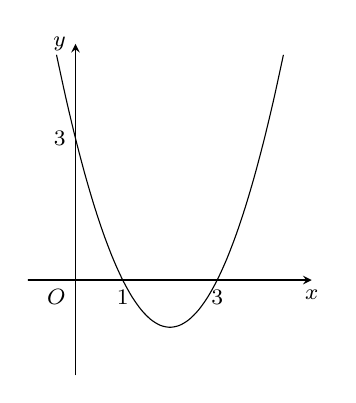
\begin{tikzpicture}[scale=0.6, font=\footnotesize, line join=round, line cap=round, >=stealth,
	declare function={
	f(\x)=(\x)^2-4*(\x)+3;}]
	\draw[->] (-1,0)--(5,0) node[below]{$x$};
	\draw[->] (0,-2)--(0,5) node[left]{$y$};
	\path (0,3) node[left]{$3$};
	\path (1,0) node[below]{$1$};
	\path (3,0) node[below]{$3$};
	\draw(0,0) node[below left]{$O$};
	\draw[smooth] plot[domain=-0.4:4.4] ({\x},{f(\x)});
	\end{tikzpicture}}
\loigiai{
	Nhìn vào đồ thị hàm số ta thấy\\
	Đồ thị hàm số cắt trục hoành tại hai điểm $M\left( 1;\,0 \right),\,N\left( 3;\,0 \right)\,\Rightarrow \,MN=2\,\Rightarrow $.
	}
\end{ex}
\begin{ex}%[0D3H1-7]%[Biên soạn tài liệu dạy học bộ KNTT-CS]%[Duong Xuan Loi]
	Nhiệt độ mặt đất đo được khoảng $30^\circ$C. Biết rằng cứ lên cao $1$ km thì nhiệt độ giảm đi $5^\circ$C. Hãy viết hàm số $t$ theo độ cao $h$ và nhiệt độ $t$ tính bằng $^\circ$C.
	\choice
	{$t=5h-30$}
	{$t=5h+30$}
	{$t=-5h-30$}
	{\True $t=30-5h$}
\loigiai{
	Hàm số $t$ theo độ cao $h$ là $t=30-5h$.
	}
\end{ex}
\Closesolutionfile{ans}
%\indapan{6}{ans/ans-c6b15-lc}
%---------------------Trắc nghiệm đúng sai
\ind{PHẦN II.} \inden{Câu trắc nghiệm đúng sai. Trong mỗi ý a), b), c), d) ở mỗi câu, học sinh chọn đúng hoặc sai.}
\setcounter{ex}{0}
\Opensolutionfile{ans}[ans/ans-c6b15-ds]
\begin{ex}%[0D3N1-3]%[Biên soạn tài liệu dạy học bộ KNTT-CS]%[Duong Xuan Loi]
	Cho hàm số $y=x^3-3x$ có đồ thị $(C)$.
	\choiceTF
	{Điểm $M(0; 1)$ thuộc đồ thị hàm số}
	{\True Tập xác định là $\mathbb{R}$}
	{\True Tập xác định là $(-\infty; +\infty)$}
	{\True Đồ thị hàm số đi qua điểm $N(1;-2)$}
\loigiai{
	\begin{itemchoice}
		\itemch Vì $y\left(0\right)=0$.
		\itemch Tập xác định là $\mathbb{R}=(-\infty; +\infty)$.
		\itemch Tập xác định là $\mathbb{R}=(-\infty; +\infty)$.
		\itemch Vì $y\left(1\right)=-2$.
	\end{itemchoice}
	}
\end{ex}
\begin{ex}%[0D3H1-4]%[Biên soạn tài liệu dạy học bộ KNTT-CS]%[Duong Xuan Loi]
	\immini{Cho hàm số $y=f(x)$ có đồ thị như hình vẽ bên. Mỗi kết quả dưới đây đúng hay sai?}{
	\begin{tikzpicture}[font=\footnotesize, line join=round, line cap=round, >=stealth,scale=1]
		\draw[->] (-2,0) -- (3,0) node[below] {$x$};
		\draw[->] (0,-3) -- (0,1.5) node[left] {$y$};
		\begin{scope}
			\clip (-2.5,-2.5) rectangle (3,2);
			\draw[samples=200,domain=-2 :5,smooth,variable=\x] plot (\x,{-(\x)^2+1*(\x)}) (-1.2,-2) node[above] {$(P)$};
		\end{scope}
		\foreach \x/\y in{0/0,1/0,2/0,0/1}{
		\fill (\x,\y) circle(1.5pt);
		}
		\path
		node at (0,0)[above left]{$O$}
		node at (1,0)[below left]{$1$}
		node at (2,0)[below]{$2$}
		node at (0,1)[left]{$1$};
	\end{tikzpicture}
	}
	\choiceTF
	{\True $f(x)=0\Leftrightarrow \hoac{&x=0\\&x=1}$}
	{$f(0)=1$}
	{\True Hàm số đồng biến trên $\left(-\infty;0\right)$}
	{$1\le f(x)$, $\forall x\in\mathscr{D}$}
\loigiai{
	\begin{itemchoice}
		\itemch Đồ thị hàm số $y=f(x)$ cắt trục hoành tại hai điểm có hoành độ $x=0$ và $x=1$.
		\itemch Từ đồ thị hàm số $y=f(x)$ thì $f(0)=0$.
		\itemch Từ đồ thị của hàm số suy ra hàm số đồng biến trên $\left(-\infty;0\right)$.
		\itemch Từ đồ thị ta có $f(x)<1$.
	\end{itemchoice}
	}
\end{ex}
\begin{ex}%[0D3H1-7]%[Biên soạn tài liệu dạy học bộ KNTT-CS]%[Duong Xuan Loi]
	Giả sử giá điện sinh hoạt trong mỗi tháng dành cho các hộ gia đình được cho bởi bảng sau
	\begin{center}
		\begin{tabular}{|c|c|}
			\hline
			Mức kWh điện tiêu thụ  & Giá bán điện (VNĐ/ kWh) \\
			\hline
			Mức 1: từ $0$ đến $100$ kWh  & $1\,600$\\
			\hline
			Mức 2: từ trên $100$ đến $300$ kWh  & $2\,000$\\
			\hline
			Mức 3: trên $300$ kWh  & $3\,000$\\
			\hline
		\end{tabular}
	\end{center}
	\choiceTF
	{\True Nếu hộ gia đình tiêu thụ $50$ kWh thì số tiền phải trả là $80\,000$ VNĐ}
	{Biểu thức biểu diễn số tiền phải trả theo số tiêu thụ điện $x$ là $f(x)=2\,000x+20\,000$}
	{\True Số tiền điện một tháng là $420\,000$ VNĐ thì số điện tiêu thụ là $230$ kWh}
	{Số tiền điện một tháng tối đa để không vượt quá mức $2$ là $500\,000$ VNĐ}
\loigiai{
	\begin{itemchoice}
		\itemch Nếu hộ gia đình tiêu thụ $50$ kWh thì số tiền phải trả là $50\cdot 1\,600=80\,000$ VNĐ.
		\itemch Gọi $ x $ kWh là mức điện tiêu thụ. Khi đó, ta có công thức liên hệ giữa số kWh điện tiêu thụ và số tiền tương ứng phải trả $ f(x) $ như sau
		\allowdisplaybreaks
		\begin{eqnarray*}
			&& f(x)=\heva{&1600x &(0<x\leq 100)&\\&1600\cdot 100+2000\cdot (x-100) &(100<x\leq 300)&\\&1600\cdot 100+2000\cdot 200+3000\cdot(x-300)&(x>300)&\\} \\
			&\Leftrightarrow& f(x)=\heva{&1600x &(0<x\leq 100)&\\&2000x-40000 &(100<x\leq 300)&\\&3000x-340000 &(x>300)&.}
		\end{eqnarray*}
		\itemch
		Để xác định số tiền điện là $ 420000 $ VNĐ mà hộ gia đình phải trả tương ứng với số kWh điện tiêu thụ bao nhiêu, ta cần xác định công thức tương ứng.\\
		Với $ f(x)=1600x $, $ 0<x\leq 100 $ thì $ 0<f(x)\leq 160000 $.\\
		Với $ f(x)=2000x-40000 $, $ 100<x\leq 300 $ thì $ 160000<f(x)\leq 560000 $.\\
		Với $ f(x)=3000x-340000 $, $ x>300 $ thì $ f(x)>560000 $.\\
		Vì $ 160000<420000<560000 $ nên ứng với số tiền điện $ 420000 $ VNĐ thì số kWh điện tiêu thụ của hộ gia đình đó là \[ \dfrac{420000+40000}{2000}=230 \text{ kWh.}\]
		Vậy số kWh điện tiêu thụ của hộ gia đình đó là $ 230 $ kWh.
		\itemch Số tiền điện một tháng tối đa để không vượt quá mức 2 là $560000$ VNĐ.
	\end{itemchoice}
	}
\end{ex}
\begin{ex}%[0D3H1-7]%[Biên soạn tài liệu dạy học bộ KNTT-CS]%[Duong Xuan Loi]
	Một hiệu chuyên cho thuê xe máy niêm yết giá như sau: Giá thuê xe là $110$ nghìn đồng một ngày cho ba ngày đầu tiên và $80$ nghìn đồng cho mỗi ngày tiếp theo.
	\choiceTF
	{\True Tổng số tiền phải trả T (nghìn đồng) theo số ngày $x$ được xác định bởi $T(x)=80x+90$ nếu $x>3$}
	{$T(2)=230$}
	{\True Với số tiền là $2$ triệu đồng thì thuê xe tối đa trong $22$ ngày liên tiếp}
	{$T(x)$ là hàm đồng biến $\left(0;+\infty\right)$}
\loigiai{
	\begin{itemchoice}
		\itemch Ta có $T(x)=\heva{& 110x & \text{nếu}\,0\le x\le 3\\& 80x+90 & \text{nếu}\, x>3.}$
		\itemch $T(2)=110\cdot 2=220$ nghìn đồng.
		\itemch Với $0\le x \le 3$ thì $ 110x\le 330$.\\
		Với $2$ triệu đồng số tiền khách còn sau khi thuê $3$ ngày đầu là $2000-330=1670$ nghìn đồng.\\
		Xét $80x+90\le 1670\Leftrightarrow x\le 19{,}75$.\\
		Với số tiền là $2$ triệu đồng thì thuê xe tối đa trong $3+19=22$ ngày liên tiếp
		\itemch $T(x)$ là hàm số đồng biến.
	\end{itemchoice}
	}
\end{ex}
\Closesolutionfile{ans}
%\indapan{2}{ans/ans-c6b15-ds}
%---------------Trắc nghiệm trả lời ngắn
\ind{PHẦN III.} \inden{Câu trả lời ngắn.}
\setcounter{ex}{0}
\Opensolutionfile{ans}[ans/ans-c6b15-kq]
\begin{ex}%[0D3H1-3]%[Biên soạn tài liệu dạy học bộ KNTT-CS]%[Duong Xuan Loi]
	Cho hàm số $f(x)=\heva{&x+\sqrt{x-2},\,\,\text{khi}\,\,x\ge 2\\&1-3x,\,\,\,\text{khi}\,\,x<2}$. Giá trị $f(1)$ bằng
	\par\shortans[oly]{$-2$}
\loigiai{
	Với $x=1<2$ suy ra $f(1)=1-3\cdot1=-2$.
	}
\end{ex}
\begin{ex}%[0D3H1-3]%[Biên soạn tài liệu dạy học bộ KNTT-CS]%[Duong Xuan Loi]
	Cho hàm số $f(x) = \heva{&\dfrac{2\sqrt{x - 2} - 3}{x - 1} \;\; \text{khi} \;\; x \geq 2 \\& x^2 + 2 \text  \;\; \text{khi} \;\; x < 2}$. Tính $P = f(2) + f(-2)$.
	\par\shortans[oly]{$6$}
\loigiai{
	Ta có $\heva{&f(2) = \dfrac{2\sqrt{2 - 2} - 3}{2 - 1} = 0\\&f(-2) = (-2)^2 + 2 = 6} $. Suy ra $P = f(2) + f(-2) = 6$.
	}
\end{ex}
\begin{ex}%[0D3V1-5]%[Biên soạn tài liệu dạy học bộ KNTT-CS]%[Duong Xuan Loi]
	Tổng tất cả các giá trị nguyên dương của tham số $m$ để hàm số $y=-2 x^2+(m+1) x+3$ nghịch biến trên khoảng $(1 ; 5)$ là
	\par\shortans[oly]{$6$}
\loigiai{
	Ta có hoành độ đỉnh $ \dfrac{-b}{2a}=\dfrac{m+1}{4} $.\\
	Để hàm số nghịch biến trên khoảng $ (1;5) $ thì $ \dfrac{m+1}{4} \le 1 \Leftrightarrow m \le 3 $.\\
	Suy ra các giá trị nguyên dương của $m$ thỏa là $ 1 $, $ 2 $, $ 3 $.\\
	Tổng các giá trị của $ m $ là $ 1+2+3=6 $.
	}
\end{ex}
\begin{ex}%[0D3V1-2]%[Biên soạn tài liệu dạy học bộ KNTT-CS]%[Duong Xuan Loi]
	Tập hợp $S$ là tập hợp chứa các số nguyên dương $m$ để hàm số $y=\sqrt{m-x}+\sqrt{x-2m+5}$ có tập xác định là một đoạn có độ dài không nhỏ hơn $3$. Tính tổng bình phương các phần tử của $S$?
	\par\shortans[oly]{$5$}
\loigiai{
	Hàm số xác định khi và chỉ khi $\heva{&m-x\ge 0\,\,\,\,\,\,\,\,\\&x-2m+5\ge 0} \Leftrightarrow \heva{&x\le m\,\,\,\,\,\,\,\,\\&x\ge 2m-5.}$\\
	TXĐ của hàm số là một đoạn có độ dài không nhỏ hơn $3$ khi và chỉ khi \[\heva{&m>2m-5\\&m-2m+5\ge 3} \Leftrightarrow \heva{&m<5\\&m\le 2} \Leftrightarrow m\le 2.\]
	Với $m\in\mathbb{Z}$, $m>0$, suy ra $m\in\left\{1;2\right\}$. Vậy có $1^2+2^2=5$.
	}
\end{ex}
\begin{ex}%[0D3V1-7]%[Biên soạn tài liệu dạy học bộ KNTT-CS]%[Duong Xuan Loi]
	Giá thuê xe ô tô tự lái là $ 1{,}2 $ triệu đồng một ngày cho hai ngày đầu tiên và $ 900 $ nghìn đồng cho mỗi ngày tiếp theo. Giá thêu xe trong $5$ ngày là bao nhiêu triệu đồng?
	\shortans[oly]{$4{,}5$}
\loigiai{
	\begin{itemize}
		\item Công thức của hàm số đã cho là
		\[ T=T(x)=\heva{&1{,}2 x\quad\text{ nếu } 1\leq x\leq 2\\ &0{,}9 x\quad\text{ nếu } x>2.}\]
		\item Giá thêu xe trong $5$ ngày là $ T(5)=0{,}9\cdot 5=4{,}5 $.
	\end{itemize}
	}
\end{ex}
\begin{ex}%[0D3C1-7]%[Biên soạn tài liệu dạy học bộ KNTT-CS]%[Duong Xuan Loi]
	Quan sát bảng giá nước sinh hoạt cho hộ gia đình năm $2\,022$ tại Hà Nội
	\begin{center}
		\begin{tabular}{|c|c|c|c|c|c|}
			\hline
			STT & Mức sử dụng nước sinh & Giá bán & Thuế & Phí bảo vệ môi & Giá thanh \\
			& hoạt của dân cư  & nước (VND) & GTGT ($5\%$) & trường ($10\%$) & toán (VND) \\
			& (m$^3$/tháng/gia đình)        &              &              &                 & \\
			\hline
			1 & $10$ m$^3$ đầu tiên & $5\,973$ & $298{,}65$ & $597{,}30$ & $6\,869$ \\
			\hline
			2 & Từ trên $10$ m$^3$ đến $20$ m$^3$ & $7\,052$ & $352{,}50$ & $705{,}20$ & $8\,110$ \\
			\hline
			3 & Từ trên $20$ m$^3$ đến $30$ m$^3$ & $8\,669$ & $433{,}45$ & $866{,}90$ & $9\,969$ \\
			\hline
			4 & Trên $20$ m$^3$ & $15\,929$ & $796{,}45$ & $1\,592{,}90$ & $18\,318$ \\
			\hline
		\end{tabular}
	\end{center}
	Số tiền phải trả khi sử dụng $25$ m$^3$ trong tháng $8$ năm $2\,022$ bao nhiêu nghìn đồng (kết quả làm tròn đến hàng nghìn).
	\shortans[oly]{$200$}
\loigiai{
	Tính số tiền phải trả khi sủ dụng $25$ m$^3$ trong tháng $8$ năm $2022$.\\
	Do số khối nước tiêu thụ là $25$ m$^3$ nên số tiền được tính theo ba bậc\\
	Bậc 1: Số tiền phải trả cho $10$ m$^3$ nước đầu tiên là $6\,869$\\
	Bậc 2: Số tiền phải trả cho $10$ m$^3$ tiếp theo ở bậc $2$ là $8\,110$\\
	Bậc 3: Số tiền phải trả cho $5$ m$^3$ tiếp theo ở bậc $3$ là $9\,969$\\
	Tổng số tiền nước phải trả cho $25$ m$^3$ là $68\,690+81\,100+49\,845=199\,635\approx 200$ (nghìn đồng).
	}
\end{ex}
\Closesolutionfile{ans}
%\indapan{3}{ans/ans-c6b15-kq}
%------------------Tự luận
\ind{PHẦN IV.} \inden{Tự luận.}
\setcounter{ex}{0}
\begin{ex}%[0D3H1-2]%[Biên soạn tài liệu dạy học bộ KNTT-CS]%[Duong Xuan Loi]
	Tìm tập xác định của các hàm số sau
	\begin{listEX}[3]
		\item $ y=2x^3+3x+1 $.
		\item $ y=\dfrac{x-1}{x^2-3x+2 } $.
		\item $ y=\sqrt{x+1}+\sqrt{1-x} $.
		\item $y=\sqrt{3x-9}$.
		\item $y=\dfrac{x+2}{4-2x}$.
	\end{listEX}
\loigiai{
	\begin{enumerate}
		\item Biểu thức $ 2x^3+3x+1 $ có nghĩa với mọi $ x\in \mathbb{R} $.\\
		Vậy tập xác định của hàm số đã cho là $ \mathscr{D}=\mathbb{R} $.
		\item Biểu thức $ \dfrac{x-1}{x^2-3x+2 } $ có nghĩa khi $ x^2-3x+2\neq 0\Leftrightarrow \heva{&x\neq 1\\&x\neq 2.} $\\
		Vậy tập xác định của hàm số đã cho là $ \mathscr{D}=\mathbb{R}\setminus \{1;2\} $.
		\item Biểu thức $ y=\sqrt{x+1}+\sqrt{1-x} $ có nghĩa khi \[ \heva{&x+1\geq 0\\&1-x\geq 0}\Leftrightarrow \heva{&x\geq -1\\&x\leq 1}\Leftrightarrow -1\leq x\leq 1 .\]
		Vậy tập xác định của hàm số đã cho là $ \mathscr{D}=[-1;1]$.
		\item Biểu thức $\sqrt{3x-9}$ có nghĩa khi $3x-9\ge 0 \Leftrightarrow x\ge 3$.\\
		Vậy tập xác định của hàm số đã cho là $\mathscr{D}=[3;+\infty)$.
		\item Biểu thức $\dfrac{x+2}{4-2x}$ có nghĩa khi $4-2x\ne 0 \Leftrightarrow x\ne 2$.\\
		Vậy tập xác định của hàm số đã cho là $\mathscr{D}=\mathbb{R}\setminus\{2\}$.
	\end{enumerate}
	}
\end{ex}
\begin{ex}%[0D3H1-5]%[Biên soạn tài liệu dạy học bộ KNTT-CS]%[Duong Xuan Loi]
	Vẽ đồ thị các hàm số sau và chỉ ra các khoảng đồng biến, nghịch biến của chúng.
	\begin{listEX}[4]
		\item $ y=-2x+1 $
		\item $ y=-\dfrac{1}{2}x^2 $
		\item $ y=3x+1 $.
		\item $ y=x^2 -2x+3$.
	\end{listEX}
\loigiai{
	\begin{enumerate}
		\item $ y=-2x+1 $
		\begin{center}
			\begin{tikzpicture}[scale=.8, font=\footnotesize, line join=round, line cap=round,>=stealth]
				\def\xmin{-3} \def\xmax{3}
				\def\ymin{-3} \def\ymax{3}
				%\draw[color=gray!50,dashed] (\xmin,\ymin) grid (\xmax,\ymax);
				\draw[->] (\xmin,0)--(\xmax,0) node [below]{$x$};
				\draw[->] (0,\ymin)--(0,\ymax) node [left]{$y$};
				\node at (0,0) [below right]{$O$};
				\draw[fill=black] (0,1) circle (.5pt) node[left]{\footnotesize $1$};
				\draw[fill=black] (.5,0) circle (.5pt) node[above]{\footnotesize $\frac{1}{2}$};
				\clip (\xmin+0.1,\ymin+0.1) rectangle (\xmax-0.1,\ymax-0.1);
				\draw[smooth,samples=300,domain=-3:3] plot(\x,{-2*(\x)+1});
			\end{tikzpicture}
		\end{center}
		Hàm số đã cho nghịch biến trên $ \mathbb{R} $.
		\item $ y=-\dfrac{1}{2}x^2 $
		\begin{center}
			\begin{tikzpicture}[scale=.8, font=\footnotesize, line join=round, line cap=round,>=stealth]
				\def\xmin{-3} \def\xmax{3}
				\def\ymin{-4} \def\ymax{1}
				%\draw[color=gray!50,dashed] (\xmin,\ymin) grid (\xmax,\ymax);
				\draw[->] (\xmin,0)--(\xmax,0) node [below]{$x$};
				\draw[->] (0,\ymin)--(0,\ymax) node [left]{$y$};
				\node at (0,0) [below right]{$O$};
				\foreach \x in{2}\draw[fill=black] (\x,0) circle (.5pt) node[above]{\footnotesize $\x$};
				\draw[fill=black] (0,-2) circle (.5pt) node[left]{\footnotesize $-2$};
				\clip (\xmin+0.1,\ymin+0.1) rectangle (\xmax-0.1,\ymax-0.1);
				\draw[smooth,samples=300,domain=-3:3] plot(\x,{-.5*(\x)^2});
				\draw[dashed] (2,0)--(2,-2)--(0,-2);
			\end{tikzpicture}
		\end{center}
		Hàm số đã cho đồng biến trên $ (-\infty;0) $.\\
		Hàm số đã cho nghịch biến trên $ (0;+\infty) $.
		\item $ y=3x+1 $
		\begin{center}
			\begin{tikzpicture}[scale=.8, font=\footnotesize, line join=round, line cap=round,>=stealth]
				\def\xmin{-3} \def\xmax{3}
				\def\ymin{-3} \def\ymax{3}
				%\draw[color=gray!50,dashed] (\xmin,\ymin) grid (\xmax,\ymax);
				\draw[->] (\xmin,0)--(\xmax,0) node [below]{$x$};
				\draw[->] (0,\ymin)--(0,\ymax) node [left]{$y$};
				\node at (0,0) [below right]{$O$};
				\draw[fill=black] (0,1) circle (.5pt) node[right]{\footnotesize $1$};
				\draw[fill=black] (-.333,0) circle (.5pt) node[above left]{\footnotesize $-\frac{1}{3}$};
				\clip (\xmin+0.1,\ymin+0.1) rectangle (\xmax-0.1,\ymax-0.1);
				\draw[smooth,samples=300,domain=-3:3] plot(\x,{3*(\x)+1});
			\end{tikzpicture}
		\end{center}
		Hàm số đã cho đồng biến trên $ \mathbb{R}$.
		\item $ y=x^2-2x+3$
		\begin{center}
			\begin{tikzpicture}[scale=.8, font=\footnotesize, line join=round, line cap=round,>=stealth]
				\def\xmin{-2} \def\xmax{4}
				\def\ymin{-1} \def\ymax{6}
				%	\draw[color=gray!50,dashed] (\xmin,\ymin) grid (\xmax,\ymax);
				\draw[->] (\xmin,0)--(\xmax,0) node [below]{$x$};
				\draw[->] (0,\ymin)--(0,\ymax) node [left]{$y$};
				\node at (0,0) [below right]{$O$};
				\foreach \x in{1,2}\draw[fill=black] (\x,0) circle (.5pt) node[below]{\footnotesize $\x$};
				\draw[fill=black] (0,2) circle (.5pt) node[left]{\footnotesize $2$};
				\draw[fill=black] (0,3) circle (.5pt) node[left]{\footnotesize $3$};
				\clip (\xmin+0.1,\ymin+0.1) rectangle (\xmax-0.1,\ymax-0.1);
				\draw[smooth,samples=300,domain=-2:4] plot(\x,{(\x)^2-2*(\x)+3});
				\draw[dashed] (1,0)--(1,2)--(0,2) (2,0)--(2,3)--(0,3);
			\end{tikzpicture}
		\end{center}
		Hàm số đã cho nghịch biến trên $ (-\infty;1) $.\\
		Hàm số đã cho đồng biến trên $ (1;+\infty) $.
	\end{enumerate}
	}
\end{ex}
\begin{ex}
	Có bao nhiêu số nguyên $m\in[-2022;\,2022]$ để hàm số $y=\sqrt{m-2x}$ xác định trên khoảng $(-3;-1)$?
\loigiai{
	Hàm số xác định khi và chỉ khi $m-2x\ge 0 \Leftrightarrow x\le\dfrac{m}{2}$.\\
	TXĐ của hàm số là $\mathscr{D}=\left(-\infty;\,\dfrac{m}{2}\right]$.\\
	Hàm số xác định trên khoảng $(-3;\,-1)$ khi $(-3;\,-1)\subset\left(-\infty;\,\dfrac{m}{2}\right] \Leftrightarrow -1\le\dfrac{m}{2} \Leftrightarrow m\ge-2$.\\
	Với $m\in[-2022;\,2022]$ suy ra $m\in\left\{-2;-1;\ldots;2022\right\}$. Vậy có $2025$ số thỏa mãn.
	}
\end{ex}
\begin{ex}%[0D3V1-7]%[Biên soạn tài liệu dạy học bộ KNTT-CS]%[Duong Xuan Loi]
	Một lớp muốn thuê một chiếc xe khách cho chuyến tham quan với tổng đoạn đường cần di chuyển trong khoảng từ $ 550 $ km đến $ 600 $ km, có hai công ty được tiếp cận để tham khảo giá.\\
	Công ty $ A $ có giá khởi đầu là $ 3{,}75 $ triệu đồng cộng thêm $ 5\,000 $ đồng cho mỗi ki-lô-mét chạy xe.\\
	Công ty $ B $ có giá khởi đầu là $ 2{,}5 $ triệu đồng cộng thêm $ 7\,500 $ đồng cho mỗi ki-lô-mét chạy xe.\\
	Lớp đó nên chọn công ty nào để chi phí là thấp nhất?
\loigiai{
	Gọi $ x $	là số km lớp đó đi ($ x>0 $).\\
	Số tiền phải trả cho công ty $ A $ là $ 3{,}75+5\,000x $ (triệu đồng).\\
	Số tiền phải trả cho công ty $ B $ là $ 2{,}5+7\,500x $ (triệu đồng).\\
	Ta có $ x=600-550=50 $ km.\\
	Suy ra số tiền phải trả cho công ty $ A $ là $ 3{,}75+5\,000\cdot 50=4 $ (triệu đồng).\\
	Số tiền phải trả cho công ty $ B $ là $ 2{,}5+7\,500\cdot 50=2{,}875 $ (triệu đồng).\\
	Vậy chọn công ty $ B $ có chi phí thấp hơn.
	}
\end{ex}
\begin{ex}%[0D3V1-7]%[Biên soạn tài liệu dạy học bộ KNTT-CS]%[Duong Xuan Loi]
	Một lớp học muốn thuê một hướng dẫn viên cho chuyến tham quan, có hai công ty được liên hệ  để lấy các thông tinh về giá.
	\begin{itemize}
		\item Công ty $ A $ có phí dịch vụ ban đầu là $ 375 $  USD  cộng thêm $0{,}5 $ USD cho mỗi ki-lô-mét hướng dẫn.
		\item Công ty $ B $ có phí dịch vụ ban đầu là $ 250 $ USD cộng thêm $ 0{,}75 $ USD cho mỗi ki-lô-mét hướng dẫn.
	\end{itemize}
	\begin{enumerate}
		\item Lớp học nên chọn công ty nào để thuê hướng dẫn viên nếu biết rằng chuyến đi sẽ đến một địa điểm nào đó với tổng khoảng cách đi lại là $ 400 $ km, $ 600 $ km?
		\item Vậy nếu đi với  khoảng cách là bao nhiêu thì chọn công ty $ A $ có lợi hơn.
	\end{enumerate}
\loigiai{
	Gọi $ x $	là số km lớp đó đi ($ x>0 $).\\
	Số tiền phải trả cho công ty $ A $ là $ 375+0{,}5x $ (USD).\\
	Số tiền phải trả cho công ty $ B $ là $ 250+0{,}75x $ (USD).
	\begin{enumerate}
		\item
		\begin{itemize}
			\item 	Nếu $ x=400 $ km thì  số tiền phải trả cho công ty $ A $ là $ 375+ 0{,}5\cdot 400=575 $ (USD), số tiền phải trả cho công ty $ B $ là $ 250+0{,}75\cdot 400=550 $ (USD).\\
			Vậy chọn công ty $ B $ có lợi  hơn.
			\item 	Nếu $ x=600 $ km thì  số tiền phải trả cho công ty $ A $ là $ 375+ 0{,}5\cdot 600=675 $ (USD), số tiền phải trả cho công ty $ B $ là $ 250+0{,}75\cdot 600=700 $ (USD).\\
			Vậy chọn công ty $A $ có lợi  hơn.
		\end{itemize}
		\item Chọn công ty $ A $ có lợi hơn tức số tiền phải trả cho công ty $ A $ ít hơn số tiền phải trả cho công ty $ B $. Ta có bất phương trình $ 375+0{,}5 x< 250+0{,}75x\Leftrightarrow x<500$.\\
		Vậy chọn công ty $ A $ lợi hơn nếu tổng khoảng cách đi lại lớn hơn $ 500 $ km.
	\end{enumerate}}
\end{ex}
\begin{ex}%[0D3V1-7]%[Biên soạn tài liệu dạy học bộ KNTT-CS]%[Duong Xuan Loi]
	Cho bảng tính tiền nước (theo https://vinid.net/blog/gia-nuoc-sinh-hoat-cap-nhat-bieu-gia-nuoc-sach-moi-nhat-2020) như sau
	\begin{center}
		\begin{tabular}{|c|c|}
			\hline
			Mức nước sử dụng & Giá (m$^3$/đồng) \\
			\hline
			Từ $0$ đến $10$ m$^3$ & $5\,973$ \\
			\hline
			Từ trên $10$ đến $20$ m$^3$ & $7\,052$ \\
			\hline
			Từ trên $20$ đến $30$ m$^3$ & $8\,669$ \\
			\hline
			Từ trên $30$ m$^3$ & $15\,929$ \\
			\hline
		\end{tabular}
	\end{center}
	\begin{enumerate}
		\item Gọi $x$ là lượng nước sử dụng (đơn vị m$^3$) và $y$ là số tiền phải trả tương ứng (đơn vị nghìn đồng). Viết công thức hàm số tính số tiền sử dụng từ $0$ đến $10$ m$^3$.
		\item Tìm tập xác định, tập giá trị của hàm số, vẽ đồ thị của hàm số này?
	\end{enumerate}
\loigiai{
	\immini
	{\begin{enumerate}
	\item Công thức hàm số là $y=5,973x$ với $0\le x\le 10$.
	\item Tập xác định của hàm số là $\mathscr{D}=[0;10]$.\\
	Ta có $0\le x\le 10 \Leftrightarrow 0\le y\le 5,973\cdot 10 \Leftrightarrow 0\le y\le 59,73$.\\
	Tập giá trị của hàm số là $[0;59,73]$.\\
	Đồ thị của hàm số $y=5,973x$ trên $[0;10]$ là một đoạn thẳng.
	\end{enumerate}}
	{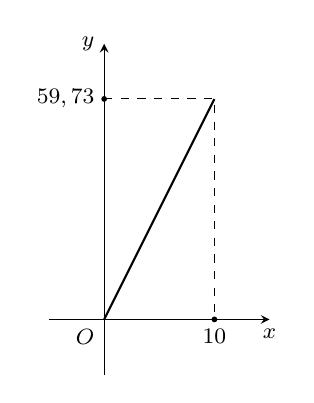
\begin{tikzpicture}[>=stealth,x=1cm,y=1cm,font=\footnotesize,scale=0.7]
	\def\a{2}
	\def\b{0}
	\draw[->] (-1,0) -- (3,0) node[below] {$x$};
	\draw[->] (0,-1) -- (0,5) node[left] {$y$};
	\draw (0,0)node[below left]{$O$};
	\fill (2,0)node[below]{$10$} circle(1.5pt);
	\fill (0,4)node[left]{$59,73$} circle(1.5pt);
	\clip (-1,-1)rectangle(3,5);
	\draw[thick,samples=150,smooth,domain=-0:2] plot(\x,{\a*\x+(\b)});
	\draw[dashed] (0,4)--(2,4)--(2,0);
	\end{tikzpicture}}
	}
\end{ex}
\Closesolutionfile{ans}